\chapter{Badania}
\label{chapter:research}

W~rozdziale tym zostały zaprezentowane wyniki badań przeprowadzone dla przykładowych funkcji referencyjnych.
Wszystkie funkcje opisane w~tym rozdziale,
ale nie załączone bezpośrednio,
znajdują się w~załącznikach niniejszej pracy dyplomowej.

\section{Przykład funkcji ,,Filtr f5''}

Przykładem potwierdzającym skuteczność algorytmu opracowanego w~ramach niniejszej pracy
może być układ arytmetyki rozproszonej \cite{memory-capacity} ,,filtru f5'' \cite{nine-filters}.
Reprezentacja tego układu za pomocą w~pełni określonych funkcji boolowskich
jest opisana tablicą o~11 zmiennych wejściowych i~11 wyjściach.
Implementacja tego układu \cite{redukcja-kompresja} w~strukturze Virtex-7 wykonana za pomocą programu Vivado 2015.4.2
wymaga zastosowania 531 komórek (330 6-wejściowych, 86 5-wejściowych; pozostałe 4, 3 i~2-wejściowe).
Opracowany algorytm redukcji i~kompresji argumentów (dalej nazywany algorytmem RedKomp)
redukuje tę funkcję do 7 argumentów,
umożliwiając jej realizację
(wykonywana w~tej samej strukturze programem Vivado)
w~strukturze zajmującej 9 komórek 6-wejściowych oraz po jednej 5, 4 i~2-wejściowej.

\section{Przykład Sasao}

Eksperyment opisany w~tym rozdziale dotyczy generatora indeksów analizowanego w~referacie Sasao \cite{sasao-workshop}.
Dla funkcji przedstawionej w~tableli \ref{sasao-a} profesor Sasao wyznaczył 5-argumentowy redukt – tabela \ref{sasao-b}.
Dzięki zastosowaniu program RedKomp udało się ten wynik poprawić uzyskując redukt 4-argumentowy,
przedstawiony w~tabeli \ref{sasao-c}.

\begin{table}[t]
\caption{Przykład funkcji generatora indeksów Sasao \cite{sasao-workshop}}
\begin{subtable}{.64\linewidth}
\caption{Pełna wersja}
\label{sasao-a}
\begin{tabular}{|r@{}c@{}c@{}c@{}c@{}c@{}c@{}c@{}c@{}c@{}c@{}c@{}c@{}c@{}c@{}c@{}c@{}c@{}c@{}c@{}c@{}c@{}c@{}c@{}c@{}c@{}c@{}c@{}c@{}c@{}c@{}c@{}c@{}c@{}c@{}c@{}c@{}c@{}c@{}c|l|}
\hline
0 & 1 & 1 & 0 & 0 & 0 & 0 & 1 & 0 & 0 & 0 & 1 & 0 & 0 & 0 & 0 & 1 & 0 & 1 & 0 & 0 & 1 & 1 & 0 & 0 & 0 & 0 & 1 & 0 & 0 & 0 & 1 & 0 & 0 & 0 & 0 & 1 & 0 & 1 & 0   &   1 \\
0 & 1 & 0 & 1 & 1 & 1 & 1 & 1 & 0 & 1 & 1 & 0 & 1 & 0 & 1 & 0 & 0 & 0 & 1 & 1 & 0 & 1 & 0 & 1 & 1 & 1 & 1 & 1 & 0 & 1 & 1 & 0 & 1 & 0 & 1 & 0 & 0 & 0 & 1 & 1   &   2 \\
1 & 1 & 1 & 1 & 0 & 1 & 0 & 1 & 0 & 1 & 1 & 1 & 0 & 1 & 1 & 1 & 0 & 0 & 0 & 0 & 1 & 1 & 1 & 1 & 0 & 1 & 0 & 1 & 0 & 1 & 1 & 1 & 0 & 1 & 1 & 1 & 0 & 0 & 0 & 1   &   3 \\
0 & 0 & 0 & 1 & 1 & 1 & 1 & 0 & 0 & 0 & 0 & 1 & 0 & 0 & 0 & 1 & 0 & 1 & 1 & 1 & 0 & 0 & 0 & 1 & 1 & 1 & 1 & 0 & 0 & 0 & 0 & 1 & 0 & 0 & 0 & 1 & 0 & 1 & 1 & 1   &   4 \\
0 & 0 & 1 & 1 & 1 & 1 & 0 & 0 & 0 & 0 & 0 & 0 & 0 & 1 & 0 & 0 & 0 & 1 & 0 & 1 & 0 & 0 & 1 & 1 & 1 & 1 & 0 & 0 & 0 & 0 & 0 & 0 & 0 & 1 & 0 & 0 & 0 & 1 & 0 & 1   &   5 \\
0 & 1 & 1 & 1 & 0 & 0 & 1 & 0 & 0 & 1 & 0 & 0 & 0 & 1 & 0 & 0 & 1 & 0 & 0 & 1 & 0 & 1 & 1 & 1 & 0 & 0 & 1 & 0 & 0 & 1 & 0 & 0 & 0 & 1 & 0 & 0 & 1 & 0 & 0 & 1   &   6 \\
0 & 0 & 1 & 0 & 0 & 0 & 1 & 1 & 1 & 0 & 0 & 0 & 1 & 1 & 1 & 1 & 0 & 0 & 1 & 0 & 0 & 0 & 1 & 0 & 0 & 0 & 1 & 1 & 1 & 0 & 0 & 0 & 1 & 1 & 1 & 1 & 0 & 0 & 1 & 0   &   7 \\
1 & 1 & 1 & 1 & 1 & 1 & 1 & 1 & 1 & 1 & 0 & 1 & 0 & 0 & 0 & 1 & 1 & 1 & 1 & 0 & 0 & 0 & 1 & 0 & 0 & 0 & 1 & 1 & 1 & 0 & 0 & 0 & 1 & 1 & 1 & 1 & 0 & 0 & 1 & 0   &   8 \\
1 & 1 & 1 & 0 & 1 & 1 & 1 & 0 & 0 & 0 & 1 & 1 & 0 & 0 & 0 & 1 & 0 & 1 & 1 & 0 & 1 & 1 & 1 & 0 & 1 & 1 & 1 & 0 & 0 & 0 & 1 & 1 & 0 & 0 & 0 & 1 & 0 & 1 & 1 & 0   &   9 \\
1 & 0 & 1 & 0 & 0 & 0 & 0 & 1 & 1 & 0 & 1 & 0 & 0 & 1 & 0 & 0 & 0 & 0 & 1 & 1 & 1 & 0 & 1 & 0 & 0 & 0 & 0 & 1 & 1 & 0 & 1 & 0 & 0 & 1 & 0 & 0 & 0 & 0 & 1 & 1   &   10 \\
\hline
\end{tabular}
\end{subtable}
\begin{subtable}{.12\linewidth}
\caption{Sasao}
\label{sasao-b}
\begin{tabular}{|r@{}c@{}c@{}c@{}l|}
\hline
0 & 1 & 1 & 0 & 0 \\
0 & 1 & 0 & 1 & 1 \\
1 & 1 & 1 & 1 & 1 \\
0 & 0 & 0 & 1 & 1 \\
0 & 0 & 1 & 1 & 1 \\
0 & 1 & 1 & 1 & 1 \\
0 & 0 & 1 & 0 & 0 \\
1 & 1 & 1 & 1 & 0 \\
1 & 1 & 1 & 0 & 0 \\
1 & 0 & 1 & 0 & 1 \\
\hline
\end{tabular}
\end{subtable}
\begin{subtable}{.16\linewidth}
\caption{RedKomp}
\label{sasao-c}
\begin{tabular}{|r@{}c@{}c@{}l|}
\hline
1 & 0 & 0 & 0 \\
0 & 0 & 0 & 0 \\
1 & 0 & 1 & 0 \\
0 & 0 & 1 & 0 \\
1 & 1 & 0 & 0 \\
1 & 1 & 1 & 1 \\
0 & 0 & 1 & 1 \\
0 & 1 & 0 & 0 \\
0 & 1 & 0 & 1 \\
0 & 0 & 0 & 1 \\
\hline
\end{tabular}
\end{subtable}
\end{table}

Rezultatem tego wyniku jest możliwość zrealizowania tej funkcji w~strukturze zaproponowanej w~referacie Sasao (rysunek \ref{fig:sasao-structure}) \cite{sasao-workshop},
zbudowanej z~dwóch pamięci: pamięć głównej i~pomocniczej,
które mają zaledwie 4 wejścia adresowe.

\begin{figure}[H]
\centering
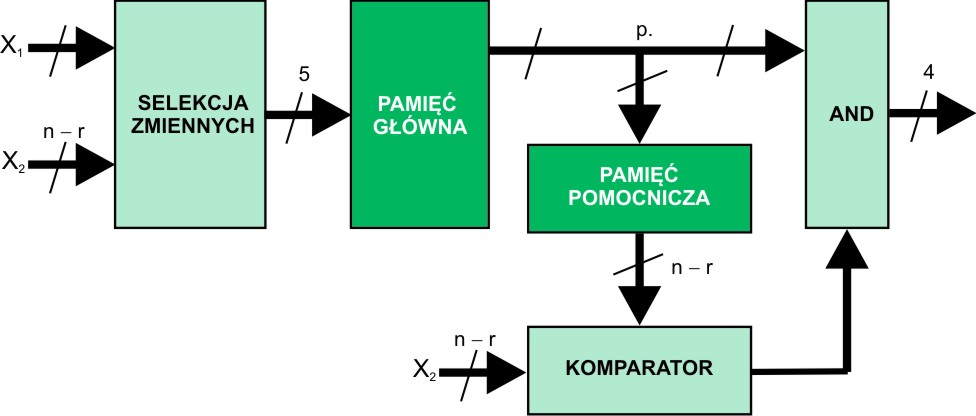
\includegraphics[width = 13cm]{chapter04/sasao-structure.jpg}
\caption{Struktura zaproponowana w~referacie Sasao (źródło \cite{sasao-workshop}).}
\label{fig:sasao-structure}
\end{figure}

W~strukturze tej blok selekcji zmiennych wybiera spośród wszystkich zmiennych $X$ podzbiór $X_1$,
reprezentujący minimalną liczbę zmiennych,
niezbędną do realizowania funkcji generowania indeksów.
Przez $r$ na rysunku została oznaczona liczność reduktu.
Jest to jednocześnie liczba wejść do pamięci głównej.
Na wyjściach pamięci głównej pojawia się indeks wektora wejściowego. % $X = X_1 \cup X_2$.
Jest on reprezentowany wektorem binarnym o~liczbie bitów $p = \lceil log_2 (k+1)\rceil$.
Indeks ten jest poprawnym indeksem wektora wejściowego wtedy,
gdy jest to wektor poszukiwany.
W~przeciwnym przypadku na wyjściach pamięci głównej pojawi się zarezerwowana na tą sytuację wartość domyślna,
na przykład wektor samych zer.
Ta wartość nie pojawi się jednak na wyjściach generatora.
Za pomocą pamięci pomocniczej i~komparatora,
przeprowadzane jest sprawdzenie,
czy pozostałe zmienne należące do zbioru $X_2$ ($X_2 = X \backslash X_1$) są zgodne ze wzorcem.
Z~pamięci pomocniczej podawane są na wejście komparatora wzorcowe wektory.
Są one porównywane tam z~rzeczywistym wektorem $X_2$ podawanym na drugie wejście komparatora.
Oczywiście wektor pobrany z~pamięci pomocniczej będzie różny od rzeczywistego wektora $X_2$ w~przypadku,
gdy nie należy on do wektora rejestrowanego.
Wtedy komparator sygnałem wyjściowym 0 zablokuje pojawienie się na wyjściach bramy AND wektora wytworzonego w~pamięci głównej.

\section{Permutacje ,,1 z~10''}

Eksperyment opisany w~tym rozdziale dotyczy funkcji ,,1 z~10'' (tabela \ref{1of10}) analizowanej w~artykule \cite{sasao-s-min}.
Funkcja ta jest redukowalna do 9 zmiennych na wiele sposobów.
Jednym z~nich jest usunięcie z~funkcji nadmiarowego argumentu $x_2$.
Funkcję po usunięciu tego argumentu i~zmianie oznaczeń na $a_1, ..., a_9$ przedstawiono w~tabeli \ref{1of10-reduct}

Przy tych oznaczeniach Sasao,
stosując algorytm 2-Min,
a~następnie 3-Min obliczył dekompozycję 5-bitową \cite{sasao-s-min}.
Została ona przedstawiona w~tabeli \ref{1of10-reduct-b}.
Rezultat uzyskany metodą RedKomp jest 4-bitowy (tabela \ref{1of10-reduct-c}).
\begin{multline} \\
b_1 = a_1 \oplus a_2 \oplus a_4 \oplus a_5, \\
b_2 = a_4 \oplus a_5 \oplus a_7 \oplus a_8, \\
b_3 = a_2 \oplus a_3 \oplus a_5 \oplus a_6, \\
b_4 = a_5 \oplus a_6 \oplus a_8 \oplus a_9. \\
\end{multline}

\begin{table}[t]
\caption{Funkcja 1 z 10 \cite{sasao-s-min}.}
\label{1of10}
\begin{tabular}{|r|ccccc ccccc|ccc ccl|}
\hline
$F$ & $x_1$ & $x_2$ & $x_3$ & $x_4$ & $x_5$ & $x_6$ & $x_7$ & $x_8$ & $x_9$ & $x_{10}$ & $y_1$ & $y_2$ & $y_3$ & $y_4$ & $y_5$ & $y_6$ \\
\hline
1 & 1 & 0 & 0 & 0 & 0 & 0 & 0 & 0 & 0 & 0 & 1 & 0 & 0 & 0 & 0 & 0 \\
2 & 0 & 1 & 0 & 0 & 0 & 0 & 0 & 0 & 0 & 0 & 0 & 0 & 0 & 0 & 0 & 0 \\
3 & 0 & 0 & 1 & 0 & 0 & 0 & 0 & 0 & 0 & 0 & 0 & 1 & 1 & 0 & 0 & 0 \\
4 & 0 & 0 & 0 & 1 & 0 & 0 & 0 & 0 & 0 & 0 & 0 & 0 & 0 & 1 & 1 & 0 \\
5 & 0 & 0 & 0 & 0 & 1 & 0 & 0 & 0 & 0 & 0 & 0 & 0 & 0 & 0 & 0 & 1 \\
6 & 0 & 0 & 0 & 0 & 0 & 1 & 0 & 0 & 0 & 0 & 1 & 0 & 0 & 0 & 0 & 1 \\
7 & 0 & 0 & 0 & 0 & 0 & 0 & 1 & 0 & 0 & 0 & 0 & 1 & 0 & 0 & 0 & 0 \\
8 & 0 & 0 & 0 & 0 & 0 & 0 & 0 & 1 & 0 & 0 & 0 & 0 & 0 & 1 & 0 & 0 \\
9 & 0 & 0 & 0 & 0 & 0 & 0 & 0 & 0 & 1 & 0 & 0 & 0 & 1 & 0 & 0 & 0 \\
0 & 0 & 0 & 0 & 0 & 0 & 0 & 0 & 0 & 0 & 1 & 0 & 0 & 0 & 0 & 1 & 0 \\
\hline
\end{tabular}
\end{table}
\begin{table}[H]
\caption{Optymalizowana funkcja ,,1 z~10'' \cite{sasao-s-min}.}
\begin{subtable}{.64\linewidth}
\caption{Po redukcji}
\label{1of10-reduct}

\begin{tabular}{|r|c@{}c@{}c@{}c@{}c@{}c@{}c@{}c@{}c|c@{}c@{}c@{}c@{}c@{}l|}
\hline
$F$ & $a_1$ & $a_2$ & $a_3$ & $a_4$ & $a_5$ & $a_6$ & $a_7$ & $a_8$ & $a_9$ & $y_1$ & $y_2$ & $y_3$ & $y_4$ & $y_5$ & $y_6$ \\
\hline
1 & 1 & 0 & 0 & 0 & 0 & 0 & 0 & 0 & 0 & 1 & 0 & 0 & 0 & 0 & 0 \\
2 & 0 & 0 & 0 & 0 & 0 & 0 & 0 & 0 & 0 & 0 & 0 & 0 & 0 & 0 & 0 \\
3 & 0 & 1 & 0 & 0 & 0 & 0 & 0 & 0 & 0 & 0 & 1 & 1 & 0 & 0 & 0 \\
4 & 0 & 0 & 1 & 0 & 0 & 0 & 0 & 0 & 0 & 0 & 0 & 0 & 1 & 1 & 0 \\
5 & 0 & 0 & 0 & 1 & 0 & 0 & 0 & 0 & 0 & 0 & 0 & 0 & 0 & 0 & 1 \\
6 & 0 & 0 & 0 & 0 & 1 & 0 & 0 & 0 & 0 & 1 & 0 & 0 & 0 & 0 & 1 \\
7 & 0 & 0 & 0 & 0 & 0 & 1 & 0 & 0 & 0 & 0 & 1 & 0 & 0 & 0 & 0 \\
8 & 0 & 0 & 0 & 0 & 0 & 0 & 1 & 0 & 0 & 0 & 0 & 0 & 1 & 0 & 0 \\
9 & 0 & 0 & 0 & 0 & 0 & 0 & 0 & 1 & 0 & 0 & 0 & 1 & 0 & 0 & 0 \\
0 & 0 & 0 & 0 & 0 & 0 & 0 & 0 & 0 & 1 & 0 & 0 & 0 & 0 & 1 & 0 \\
\hline
\end{tabular}

\end{subtable}
\begin{subtable}{.12\linewidth}
\caption{Sasao}
\label{1of10-reduct-b}

\begin{tabular}{|r@{}c@{}c@{}c@{}l|}
\hline
  &   &   &   &   \\
\hline
1 & 0 & 0 & 0 & 0 \\
0 & 0 & 0 & 0 & 0 \\
0 & 1 & 1 & 0 & 1 \\
0 & 0 & 1 & 1 & 0 \\
0 & 0 & 0 & 0 & 1 \\
1 & 0 & 0 & 0 & 1 \\
0 & 1 & 0 & 0 & 0 \\
0 & 0 & 0 & 1 & 0 \\
0 & 0 & 1 & 0 & 1 \\
0 & 0 & 1 & 0 & 0 \\
\hline
\end{tabular}

\end{subtable}
\begin{subtable}{.16\linewidth}
\caption{RedKomp}
\label{1of10-reduct-c}

\begin{tabular}{|r@{}c@{}c@{}l|}
\hline
$b_1$ & $b_2$ & $b_3$ & $b_4$ \\
\hline
1 & 0 & 0 & 0 \\
0 & 0 & 0 & 0 \\
1 & 0 & 1 & 0 \\
0 & 0 & 1 & 0 \\
1 & 1 & 0 & 0 \\
1 & 1 & 1 & 1 \\
0 & 0 & 1 & 1 \\
0 & 1 & 0 & 0 \\
0 & 1 & 0 & 1 \\
0 & 0 & 0 & 1 \\
\hline
\end{tabular}

\end{subtable}
\end{table}


\section{Permutacje ,,2 z~16''}

Eksperyment opisany w~tym rozdziale dotyczy funkcji ,,2 z~16''.
Dekompozycja liniowa tej funkcji obliczana algorytmem 2-Min oraz 3-Min \cite{sasao-s-min} tworzy układ o~11 wejściach.
Liczby wejść do poszczególnych bramek XOR nie są podane.
Program RedKomp umożliwia realizację tej funkcji na pamięci o~9 wejściach adresowych.
Poszczególne wejścia $a_1$ do $a_9$ tej pamięci są wyrażone następującymi funkcjami XOR:
\begin{multline} \\
a_1 = x_8 \oplus x_2 \oplus x_3, \\
a_2 = x_{11} \oplus x_3 \oplus x_4, \\
a_3 = x_{14} \oplus x_7 \oplus x_8, \\
a_4 = x_{15} \oplus x_{10} \oplus x_{11}, \\
a_5 = x_{10} \oplus x_{11} \oplus x_{13} \oplus x_{14}, \\
a_6 = x_1 \oplus x_2 \oplus x_4 \oplus x_5, \\
a_7 = x_4 \oplus x_5 \oplus x_6 \oplus x_7, \\
a_8 = x_6 \oplus x_7 \oplus x_9 \oplus x_{10}, \\
a_9 = x_9 \oplus x_{10} \oplus x_{12} \oplus x_{13}. \\
\end{multline}

\section{Permutacje ,,2 z~20''}

Eksperyment opisany w~tym rozdziale dotyczy funkcji ,,2 z~20''.
Dekompozycja liniowa tej funkcji obliczana algorytmem 2-Min oraz 3-Min \cite{sasao-s-min} tworzy układ o~14 wejściach.
Liczby wejść do poszczególnych bramek XOR nie są podane.
Program RedKomp umożliwia realizację tej funkcji na pamięci o~9 wejściach adresowych.
Poszczególne wejścia $a_1$ do $a_9$ tej pamięci są następującymi funkcjami XOR:

\begin{multline} \\
a_1 = x_{4} \oplus x_{5} \oplus x_{10} \oplus x_{11} \oplus x_{13} \oplus x_{14}, \\
a_2 = x_{11} \oplus x_{3} \oplus x_{4} \oplus x_{16} \oplus x_{17}, \\
a_3 = x_{16} \oplus x_{17} \oplus x_{19} \oplus x_{1} \oplus x_{2}, \\
a_4 = x_{14} \oplus x_{7} \oplus x_{8} \oplus x_{15} \oplus x_{10} \oplus x_{11}, \\
a_5 = x_{15} \oplus x_{10} \oplus x_{11} \oplus x_{18} \oplus x_{8} \oplus x_{2} \oplus x_{3}, \\
a_6 = x_{18} \oplus x_{8} \oplus x_{2} \oplus x_{3} \oplus x_{1} \oplus x_{2} \oplus x_{4} \oplus x_{5}, \\
a_7 = x_{1} \oplus x_{2} \oplus x_{4} \oplus x_{5} \oplus x_{9} \oplus x_{10} \oplus x_{12} \oplus x_{13}, \\
a_8 = x_{9} \oplus x_{10} \oplus x_{12} \oplus x_{13} \oplus x_{12} \oplus x_{13} \oplus x_{17} \oplus x_{18}, \\
a_9 = x_{12} \oplus x_{13} \oplus x_{17} \oplus x_{18} \oplus x_{19} \oplus x_{1} \oplus x_{2} \oplus x_{6} \oplus x_{7} \oplus x_{9} \oplus x_{10}. \\
\end{multline}

Program RedKomp przeprowadza obliczenia sekwencyjnie.
Dzięki temu możliwe jest uzyskanie wyniku dekompozycji lepiej dopasowanej do potrzeb.
W~przypadku funkcji ,,2 z~20''
program RedKomp jest w~stanie zaproponować rozwiązania realizowalne na pamięciach
od 19 (obliczone w~wyniku samej redukcji argumentów) do 9 wejściach adresowych.
Dla przykładu poniżej została przedstawiona dekompozycja obliczona programem RedKomp na układ o~14 wejściach jak w~przypadku rozwiązania Sasao \cite{sasao-s-min}.
Poszczególne wejścia $b_1$ do $b_{14}$ tej pamięci są następującymi funkcjami XOR:

\begin{multline} \\
b_1 = x_{16}, \\
b_2 = x_{17}, \\
b_3 = x_{18}, \\
b_4 = x_{19}, \\
b_5 = x_{1} \oplus x_{2}, \\
b_6 = x_{4} \oplus x_{5}, \\
b_7 = x_{6} \oplus x_{7}, \\
b_8 = x_{8} \oplus x_{2} \oplus x_{3}, \\
b_9 = x_{9} \oplus x_{10}, \\
b_{10} = x_{11} \oplus x_{3} \oplus x_{4}, \\
b_{11} = x_{12} \oplus x_{13}, \\
b_{12} = x_{14} \oplus x_{7} \oplus x_{8}, \\
b_{13} = x_{15} \oplus x_{10} \oplus x_{11}, \\
b_{14} = x_{10} \oplus x_{11} \oplus x_{13} \oplus x_{14}. \\
\end{multline}
